\documentclass{article}

\usepackage[left=1.8in,right=1.8in,top=.6in,bottom=1in]{geometry}

\usepackage{assumptionsofphysics}
\usepackage{tikz}
\usepackage{hyperref}
\hypersetup{
	colorlinks=true,
	citecolor=blue,
	urlcolor=blue,
	linkcolor=blue
}
\frenchspacing

\newcommand{\marginleft}[1] {\reversemarginpar\marginpar{#1}}
\newcommand{\marginright}[1] {\normalmarginpar\marginpar{#1}}

\def\ordinals{\textbf{ORD}}
\def\cardinals{\textbf{CRD}}

\def\ordless{\prec}
\def\ordleq{\preceq}
\def\ordeq{\sim}
\def\ordgeq{\succeq}
\def\ordgtr{\succ}

\def\crdless{\sqsubset}
\def\crdleq{\hookrightarrow}
\def\crdeq{\leftrightarrow}
\def\crdgeq{\hookleftarrow}
\def\crdgtr{\sqsupset}


\title{Bare minimum: set theory}

\date{\vspace{-5ex}}
\begin{document}

\maketitle


\begin{abstract}
This note presents a condensed summary of set theory which can function as a crash course, refresher and/or reference. Bare minima are meant to give a rough overview, by no means complete, of the subject to the intellectually curious, particularly in the context of foundational questions in physics. This work is part of Assumptions of Physics (\url{https://assumptionsofphysics.org}), a project that aims to identify a handful of physical principles from which the basic laws can be rigorously derived.
\end{abstract}

Ordinal: $\ordless \ordleq \ordeq \ordgeq \ordgtr$

Cardinal: $\crdless \crdleq \crdeq \crdgeq \crdgtr$


\section{Introduction}

Set theory is important for those working on the Assumptions of Physics for at least three reasons. First, it is a foundational framework in mathematics. Second, it showcases a successful attempt at concept generalization. Third, it shows how a formal system is bootstrapped.

There are two rough branches of set theory: naive and axiomatic. Naive set theory is built on intuitive concepts, and as such is not fully formalized and is open to potential paradoxes. Axiomatic set theory provides a fully formalized axiomatic system that aims to close those problems. We will start with naive set theory, which is the best setting for defining all the basic notions and getting a sense of how the framework works. Then we will turn our attention to axiomatic set theory to get a sense of what problems it solves and how, and whether those solutions mesh with foundational goals  in physics.

TODO: cite https://www.math24.net/topics-set-theory and set theory book

\section{Naive set theory}

We take sets and elements as primitive objects, with no formal definition. A \textbf{set} $A$ is a collection of elements. If an element $e$ belongs to the set we say $e$ \textbf{is in} $A$, noted $ e 
\in A$. A set $A$ can be defined by listing the elements, noted $A = \{ e_1, e_2, e_3 \}$. A set $A$ can be defined by specifying how to build the elements through a rule (i.e. predicate) $P(e)$, and is noted $A = \{e \, | \,  P(e) \}$. The rule may include symbols like for all $\forall$, exists $\exists$, logical connectors AND $\AND$, OR $\OR$ and $\NOT$.

\begin{defn}[Common sets]
	 The \textbf{empty set}
	 \marginleft{Common sets: $\emptyset$, $\{a\}$, $\mathbb{N}$, $\mathbb{Z}$, $\mathbb{Q}$, $\mathbb{R}$, $\mathbb{C}$}
	  $\emptyset$ is the set with no elements. A \textbf{singleton} is the set of a single value $\{a\}$.
	 The \textbf{set of natural numbers} $\mathbb{N} = \{ 0, 1, 2, ... \}$. The \textbf{set of positive natural numbers} $\mathbb{N}^+ = \{n \in \mathbb{N} \, | \, n > 0\}$. The \textbf{set of integer numbers} $\mathbb{Z} = \{ ... , -2, -1, 0, +1, +2, ...\}$. The \textbf{set of rational numbers} $\mathbb{Q}$. The \textbf{set of real numbers} $\mathbb{R}$. The \textbf{set of complex numbers} $\mathbb{C}$. A \textbf{universe} $U$ is the set that, within a specific context, contains all entities under study.
\end{defn}

\subsection{Basic definitions}

\marginright{~\\
	\def\setA{ (-1,0) circle (2) }
	\def\setB{ (1,0) circle (2) }
	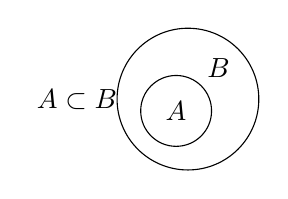
\begin{tikzpicture}[scale = 0.3]
		\draw (0,0) circle (3); 
		\draw (-0.5,-0.5) circle (1.5);
		\node at (-4.7,0) {$A \subset B$};
		\node at (-0.5,-0.5) {$A$};
		\node at (1.3,1.3) {$B$};
	\end{tikzpicture} 
}

\begin{defn}[Set relationships]
	Let $A$ and $B$ be two sets. \marginleft{Subset, superset: $\subseteq$, $\supseteq$} If all elements in $A$ are also contained in $B$, we say $A$ is a \textbf{subset} of $B$, noted $A \subseteq B$. In this case, we also say $B$ is a \textbf{superset} of $A$, noted $B \supseteq A$. Additionally, if $B$ contains elements that $A$ does not contain, we say $A$ is a \textbf{strict subset} of $B$, noted $A \subset B$, and $B$ is a \textbf{strict superset} of $A$, noted $B \supset A$. If the two sets contain exactly the same elements, then we say the sets are \textbf{equal}, noted $A = B$. If the two sets have no element in common they are said to be \textbf{disjoint}.
\end{defn}

\begin{defn}[Power set]
	Given a set $A$, its \textbf{power set}, \marginleft{Power set:\\ $\mathcal{P}(A)$, $2^{A}$} noted $\mathcal{P}(A)$ or $2^{A}$, is the set of all subsets of $A$. That is, $\mathcal{P}(A) = \{B \, | \, B \subset A \}$.
\end{defn}

\marginright{
	~\\
	\def\setA{ (-1,0) circle (2) }
	\def\setB{ (1,0) circle (2) }
	\vspace{1pt}
	\begin{tikzpicture}[scale = 0.3]
		\filldraw[black!10] \setA;
		\filldraw[black!10] \setB;
		\draw \setA; 
		\draw \setB;
		\node at (-4.7,0) {$A\!\cup \! B$};
	\end{tikzpicture} 
	\vspace{1pt}
	\begin{tikzpicture}[scale = 0.3]
		\begin{scope}
			\clip \setA;
			\filldraw[black!10] \setB;
		\end{scope}
		\draw \setA; 
		\draw \setB;
		\node at (-4.7,0) {$A\!\cap \! B$};
	\end{tikzpicture} 
	\vspace{1pt}
	\begin{tikzpicture}[scale = 0.3]
		\filldraw[black!10] \setA;
		\filldraw[white] \setB;
		\draw \setA; 
		\draw \setB;
		\node at (-4.7,0) {$A\!\setminus \! B$};
	\end{tikzpicture}
	\def\setU{ (-3,-2) rectangle (3,2) }
	\def\setA{ (0,0) circle (1.8) }
	\begin{tikzpicture}[scale = 0.3] 
		\filldraw[black!10] \setU;
		\filldraw[white] \setA;
		\draw \setU;
		\draw \setA;
		\node at (-5.3,0) {$A^{\complement}$};
	\end{tikzpicture} 
}

\begin{defn}[Set operations]
	We define \marginleft{Set operations: $\cup$, $\cap$, $\setminus$, $^{\complement}$} the following operations between two sets $A$ and $B$:
	\begin{description}
		\item[Union.]Noted $A \cup B$, the union of $A$ and $B$ is the set of all elements that are contained by $A$, $B$ or both.
		\item[Intersection.] Noted $A \cap B$, the intersection of $A$ and $B$ is the set of all elements that are contained by both.
		\item[Set difference (or relative complement).] Noted $A \setminus B$, $A$ minus $B$ is the set of all elements in $A$ that are not contained by $B$.
		\item[Complement (or absolute complement).] Noted $A^{\complement}$, represents all elements that are not contained in $A$. Note that this operation is context specific: we need to know that, within a certain context, $U$ is the set of all elements under study; then the complement of $A \subseteq U$ is $A^{\complement} = U \setminus A$.
	\end{description}

	Let $\mathcal{A} \subseteq \mathcal{P}(A)$ be a set of subsets of $A$. The operations of union $\bigcup\limits_{A \in \mathcal{A}} A$ and intersection $\bigcap\limits_{A \in \mathcal{A}} A$ can be extend to span all elements.
\end{defn}

\begin{defn}[Ordered pair]
	Given two \marginleft{Ordered pair: $(a, b)$} elements $a$ and $b$, the \textbf{ordered pair} $(a, b)$ specifies two objects in that order. That is $(a, b) \neq (b, a)$. This can be constructed setting $(a, b) = \{ \{a\}, \{a, b\}\}$.
\end{defn}

\marginright{~\\
	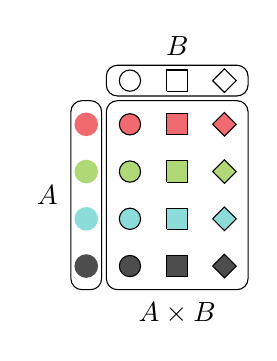
\begin{tikzpicture}[scale = 0.3] 
		\node at (-2.5,-4) {$A$};
		\node at (3,2.3) {$B$};
		\draw[rounded corners] (0,0.2) rectangle (6,1.5);
		\draw[rounded corners] (-0.2,0) rectangle (-1.5,-8);
		\draw[rounded corners] (0,0) rectangle (6,-8);
		
		\def\circlepath{circle (0.45)}
		\def\rectanglepath{ ++(-0.45,-0.45)  -- ++(0,0.9)  -- ++(0.9,0) -- ++(0,-0.9) -- ++(-0.9,0)}
		\def\diamondpath{ ++(-0.5,0)  -- ++(0.5,0.5)  -- ++(0.5,-0.5) -- ++(-0.5,-0.5) -- ++(-0.5,0.5)}
		
		% B elements
		\draw (1,0.85) \circlepath;
		\draw (3,0.85) \rectanglepath;
		\draw (5,0.85) \diamondpath;
		
		\definecolor{a}{rgb}{0.945, 0.415, 0.439}
		\definecolor{b}{rgb}{0.694, 0.847, 0.466}
		\definecolor{c}{rgb}{0.549, 0.862, 0.854}
		\definecolor{d}{rgb}{0.301, 0.301, 0.301}
		
		% A elements
		\fill[a] (-0.85, -1) circle (0.5);
		\fill[b] (-0.85, -3) circle (0.5);
		\fill[c] (-0.85, -5) circle (0.5);
		\fill[d] (-0.85, -7) circle (0.5);

		% AxB elements
		\filldraw[fill=a] (1, -1) \circlepath;
		\filldraw[fill=b] (1, -3) \circlepath;
		\filldraw[fill=c] (1, -5) \circlepath;
		\filldraw[fill=d] (1, -7) \circlepath;
		\filldraw[fill=a] (3, -1) \rectanglepath;
		\filldraw[fill=b] (3, -3) \rectanglepath;
		\filldraw[fill=c] (3, -5) \rectanglepath;
		\filldraw[fill=d] (3, -7) \rectanglepath;
		\filldraw[fill=a] (5, -1) \diamondpath;
		\filldraw[fill=b] (5, -3) \diamondpath;
		\filldraw[fill=c] (5, -5) \diamondpath;
		\filldraw[fill=d] (5, -7) \diamondpath;

		\node at (3,-9) {$A \times B$};
	\end{tikzpicture} 
}
\begin{defn}[Cartesian product]
	Given two sets \marginleft{Cartesian product: $\times$}  $A$ and $B$, the \textbf{Cartesian product} $A \times B = \{ (a,b) \, | \, \forall a \in A, b \in B \}$ is the set of all possible ordered pairs between the elements of $A$ and $B$.
\end{defn}

\begin{defn}[Disjoint union]
	Let $A$ and $B$ be two sets. The disjoint union $A \sqcup B$ is the union where the elements of the sets are always treated as distinct. That is, $A \sqcup B = \{A\} \times A \cup \{B\} \times B$.
\end{defn}

\subsection{Relations and functions}

\begin{remark}
	Relations provide a common foundation for functions (i.e. the relation is the set of pairs $(x, f(x))$), equivalences and order (i.e. the relation is the set of pairs $(a, b)$ such that $a=b$ or $a\leq b$ respectively). This is an example of highly fruitful generalization.
\end{remark}

\marginright{~\\
	\begin{tikzpicture}[scale = 0.3] 
		\node at (-2.5,-4) {$A$};
		\node at (3,2.3) {$B$};
		\draw[rounded corners] (0,0.2) rectangle (6,1.5);
		\draw[rounded corners] (-0.2,0) rectangle (-1.5,-8);
		\draw[rounded corners] (0,0) rectangle (6,-8);
		
		\def\circlepath{circle (0.45)}
		\def\rectanglepath{ ++(-0.45,-0.45)  -- ++(0,0.9)  -- ++(0.9,0) -- ++(0,-0.9) -- ++(-0.9,0)}
		\def\diamondpath{ ++(-0.5,0)  -- ++(0.5,0.5)  -- ++(0.5,-0.5) -- ++(-0.5,-0.5) -- ++(-0.5,0.5)}
		
		% B elements
		\node at (1,0.85) {
\includegraphics[scale=0.25]{cat.png}};
		\node at (3,0.85) {
\includegraphics[scale=0.25]{dog.png}};
		\node at (5,0.85) {
\includegraphics[scale=0.25]{swan.png}};
		
		\definecolor{a}{rgb}{1.0, 1.0, 1.0}
		\definecolor{b}{rgb}{1, 0.509, 0}
		\definecolor{c}{rgb}{0.45, 0.225, 0}
		\definecolor{d}{rgb}{0, 0, 0}
		
		% A elements
		\filldraw[fill=a] (-0.85, -1) circle (0.5);
		\fill[b] (-0.85, -3) circle (0.5);
		\fill[c] (-0.85, -5) circle (0.5);
		\fill[d] (-0.85, -7) circle (0.5);
		
		% AxB elements
		\node at (1, -1) {$\checkmark$};
		\node at (1, -3) {$\checkmark$};
		\node at (1, -5) {};
		\node at (1, -7) {$\checkmark$};
		\node at (3, -1) {$\checkmark$};
		\node at (3, -3) {};
		\node at (3, -5) {$\checkmark$};
		\node at (3, -7) {$\checkmark$};
		\node at (5, -1) {$\checkmark$};
		\node at (5, -3) {};
		\node at (5, -5) {};
		\node at (5, -7) {$\checkmark$};
		
		\node at (3,-9) {$R$};
	\end{tikzpicture} 
	
	\begin{tikzpicture}[scale = 0.3] 
		\node at (-2.5,-3) {$B$};
		\node at (4,2.3) {$A$};
		\draw[rounded corners] (0,0.2) rectangle (8,1.5);
		\draw[rounded corners] (-0.2,0) rectangle (-1.5,-6);
		\draw[rounded corners] (0,0) rectangle (8,-6);
		
		\def\circlepath{circle (0.45)}
		\def\rectanglepath{ ++(-0.45,-0.45)  -- ++(0,0.9)  -- ++(0.9,0) -- ++(0,-0.9) -- ++(-0.9,0)}
		\def\diamondpath{ ++(-0.5,0)  -- ++(0.5,0.5)  -- ++(0.5,-0.5) -- ++(-0.5,-0.5) -- ++(-0.5,0.5)}
		
		% B elements
		\node at (-0.85, -1) {
\includegraphics[scale=0.25]{cat.png}};
		\node at (-0.85, -3) {
\includegraphics[scale=0.25]{dog.png}};
		\node at (-0.85, -5) {
\includegraphics[scale=0.25]{swan.png}};
		
		\definecolor{a}{rgb}{1.0, 1.0, 1.0}
		\definecolor{b}{rgb}{1, 0.509, 0}
		\definecolor{c}{rgb}{0.45, 0.225, 0}
		\definecolor{d}{rgb}{0, 0, 0}
		
		% A elements
		\filldraw[fill=a] (1,0.85) circle (0.5);
		\fill[b] (3,0.85) circle (0.5);
		\fill[c] (5,0.85) circle (0.5);
		\fill[d] (7,0.85) circle (0.5);
		
		% AxB elements
		\node at (1, -1) {$\checkmark$};
		\node at (3, -1) {$\checkmark$};
		\node at (5, -1) {};
		\node at (7, -1) {$\checkmark$};
		\node at (1, -3) {$\checkmark$};
		\node at (3, -3) {};
		\node at (5, -3) {$\checkmark$};
		\node at (7, -3) {$\checkmark$};
		\node at (1, -5) {$\checkmark$};
		\node at (3, -5) {};
		\node at (5, -5) {};
		\node at (7, -5) {$\checkmark$};
		
		\node at (4,-7) {$R^{-1}$};
	\end{tikzpicture} 
	
}
\begin{defn}[Binary relation]
	Given a set $A$, \marginleft{Binary\\ relation} called \textbf{domain}, and a set $B$, called \textbf{codomain}, a \textbf{binary relation} is a set $R \subseteq A \times B$ of ordered pairs. We say $a$ is \textbf{$R$-related} to $b$, noted $aRb$ if $(a,b) \in R$. If $A=B$ (i.e. domain and codomain coincide) the relation is said \textbf{homogeneous}, \textbf{heterogeneous} if not.
\end{defn}

	
\begin{defn}[Image and preimage]
	If $X \subseteq A$, \marginleft{Image and\\ preimage} the \textbf{image of $X$ under $R$} is the set of all elements in $B$ that are related to at least one element in $X$. The \textbf{image of $R$} is set of all elements in $B$ that are related to at least one element in $A$ (i.e. the image of the full set $A$).
	
	If $Y \subseteq B$, the \textbf{preimage of $Y$ under $R$} is the set of all elements in $A$ that are related to at least one element in $Y$. The \textbf{preimage of $R$} is set of all elements in $A$ that are related to at least one element in $B$ (i.e. the preimage of the full set $B$).
\end{defn}


\begin{defn}[Converse relationship]
	Given a relationship  \marginleft{Converse: $R^{-1}$} $R$ between $A$ and $B$, the \textbf{converse} or \textbf{inverse} relationship $R^{-1}$ is the relationship where the order of the pairs is inverted. That is, $R^{-1} = \{ (b, a) \, | \, (a, b) \in R\}$.
\end{defn}

\begin{defn}[Relation properties]
	Let $R$ \marginleft{Relation properties} be a binary relation between $A$ and $B$. We define the following properties:
	\begin{description}
		\item[Functional or right-unique.] An element $a \in A$ is related to at most one element $b \in B$. That is, if $aRb$ and $cRb$ then $a = c$.
		\item[Injective or left-unique.] An element $b \in B$ is related to at most one element $a \in A$. That is, if $aRb$ and $aRc$ then $b = c$.
		\item[Serial or left-total.] Every element $a \in A$ is related to at least one element $b \in B$. That is, for each $a \in A$ there exists at least one $b \in B$ such that $aRb$. In this case, the preimage of $R$ is the whole $A$.
		\item[Surjective or right-total.] Every element $b \in B$ is related to at least one element $a \in B$. That is, for each $b \in B$ there exists at least one $a \in A$ such that $aRb$. In this case, the image of $R$ is the whole $B$.
	\end{description}
	From those basic properties, we define the following:
	\begin{description}
		\item[One-to-one.] Injective and functional (i.e. left-unique and right-unique).
		\item[One-to-many.] Injective and not functional (i.e. left-unique and not right-unique).
		\item[Many-to-one.] Not injective and functional (i.e. not left-unique and right-unique).
		\item[Many-to-many.] Not injective nor functional (i.e. not left-unique nor right-unique).
	\end{description}	
\end{defn}

\begin{defn}[Function]
	A \textbf{partial function} \marginleft{(Partial) \\ functions: \\ $f : A \to B$} $f : A \to B$ is a binary relationship between $A$ and $B$ that is functional (i.e. right-unique). The \textbf{graph} of the function $G \subset A \times B$ is the function expressed as ordered pairs. A \textbf{total function}, or simply a \textbf{function}, is a partial function that is also serial (i.e. left-total, defined on the whole domain). A function is \textbf{bijective} if it is injective and surjective.
	
	When the functional form $f(a)$ is known, this can be expressed as $a \mapsto f(a)$ (read ``$a$ maps to $f$ of $a$'').
\end{defn}

\begin{remark}
	Note that the domain and the codomain can be any set, including scalar products. Therefore $f : \mathbb{R} \times \mathbb{R} \to \mathbb{R}$ for which $(x,y) \mapsto \sqrt{x^2 + y^2}$ gives us the Euclidean norm of a two dimensional vector.
\end{remark}

\begin{defn}
	Let $f : A \to B$ be a function. This induces a relation $f : \mathcal{P}(A) \to \mathcal{P}(B)$ that associates each subset of $A$ to its image and a relation $f^{-1} : \mathcal{P}(B) \to \mathcal{P}(A)$ that associates each subset of $B$ with its reverse image.
\end{defn}

\begin{defn}[Level set]
	A level set \marginleft{Level set} of a function $f : A \to B$ is a set of where the function takes a given value $b$. In other words the reverse image $f^{-1}(\{c\})$ a singleton.
\end{defn}

\begin{prop}
	The induces relations $f : \mathcal{P}(A) \to \mathcal{P}(B)$ and $f^{-1} : \mathcal{P}(B) \to \mathcal{P}(A)$ are functions and satisfy the following properties:
	\begin{enumerate}
		\item $f(\bigcup\limits_{A \in \mathcal{A}} A) = \bigcup\limits_{A \in \mathcal{A}} f(A)$
		\item $f^{-1}(\bigcup\limits_{A \in \mathcal{A}} A) = \bigcup\limits_{A \in \mathcal{A}} f^{-1}(A)$
		\item $f^{-1}(\bigcap\limits_{A \in \mathcal{A}} A) = \bigcap\limits_{A \in \mathcal{A}} f^{-1}(A)$
	\end{enumerate}
\end{prop}

\begin{remark}
	With abuse of notation, $f$ and$f^{-1}$ indicate both the function between elements and sets. The image of the intersection is not in general the intersection of the image. Note how in both topology and measure theory continuity and measurability are defined based on the reverse images.
\end{remark}

\begin{defn}[Identity function]
	Given a set $A$, \marginleft{Identity: $\Id_A(a)$} the identity function $\Id_A : A \to A$ is the function such that $\Id_A(a) = a$ for all $a \in A$.
\end{defn}


\begin{prop}[Inverse function]
	Let $f : A \to B$ \marginleft{Inverse: $f^{-1}$} be a function. The corresponding converse relationship $f^{-1}$ is a function if and only if $f$ is bijective. In this case $f^{-1} : B \to A$ is also bijective and is called the \textbf{inverse} of $f$.
\end{prop}

\begin{defn}[Restriction]
	Let $f : A  \to B$ \marginleft{Restriction: $f|_C$} be a function and let $C \subseteq B$. Then the \textbf{restriction of $f$ over $C$} is the function $f|_C : C \to B$ such that $f|_C(c) = f(c)$.
\end{defn}

\begin{defn}[Composition]
	Let $A$, $B$ and $C$ \marginleft{Function and relation composition: $R \circ S$, $f \circ g$} be three sets. Let $R$ be a binary relationship between $A$ and $B$ and $S$ be a binary relationship between $B$ and $C$. Then the \textbf{composition of $R$ and $S$}, noted $S \circ R$, is the binary relationship between $A$ and $C$ such that $(a, c) \in S \circ R$ if we can find $b \in B$ such that $aRb$ and $bSc$.
\end{defn}

\begin{remark}
	The order of composition follows those of functions: if $f : A \to B$ and $g : B \to C$, composition leads to $c = g(f(a)) = (g \circ f)(a)$.
\end{remark}

\begin{prop}[Composition properties]
	Relation composition \marginleft{Composition properties} follows the following properties:
	\begin{itemize}
		\item Composition is associative: $R \circ (T \circ S) = (R \circ T) \circ S$
		\item Converse of composition: $(R \circ S)^{-1} = S^{-1} \circ R^{-1}$
		\item Composition of functional/injective/serial/surjective relations is \\ functional/injective/serial/surjective.
		\item If $f : A \to B$ and $g : B \to C$ are (partial) functions, then $g \circ f$ is a (partial) function.
		\item Let $f : A \to B$ is a bijective function, then $f \circ f^{-1} = \Id_B$ and $f^{-1} \circ f = \Id_A$.
	\end{itemize}
\end{prop}

\begin{defn}[Sets of functions]
	The set \marginleft{Sets of functions: $B^A$} of all possible functions $f : A \to B$ is noted $B^A$.
\end{defn}

\begin{prop}
	Let $2 = \{0, 1\}$ denote a set with two elements. Then $\mathcal{P}(A)$ and $2^A$ are in one-to-one correspondence.
\end{prop}

\begin{remark}
	The notation is due to the cardinality. If $|A| = n$ and $|B| = m$, each function is given by choosing an element of $B$ for each element of $A$, that is $m$ choices $n$ times, that is $m^n$. The power set is noted $2^A$ because each subset can be identified by a function $U : A \to \{0 , 1\}$, where $f(a)=0$ corresponds to $a \notin U$ and $f(a)=0$ corresponds to $b \in U$.
\end{remark}

TODO: add definition of set closed under operation

\subsection{Indexed families and sequences}

\begin{defn}[Families]
	An \textbf{indexed family}, \marginleft{Families, sequences: $\{x_i\}_{i \in I}$, $\{x_i\}_{i=1}^{\infty}$} or simply a \textbf{family}, $\{x_i\}_{i \in I}$ is a collection of elements identified by an \textbf{index set} $I$. More formally, an indexed family is a tuple $\langle X, I, x \rangle$ where $X$ and $I$ are sets and $x: I \to X$ is a function such that $i \mapsto x_i$. A \textbf{sequence} is an family for which the index set is a continuous interval of natural numbers. A \textbf{finite sequence} of $n$ elements is noted $\{x_i\}_{i=1}^{n}$ while an \textbf{infinite sequence} is noted $\{x_i\}_{i=1}^{\infty}$.
\end{defn}

\begin{defn}[Operations on families of sets]
	Let $\{A_i\}_{i \in I}$ \marginleft{$\bigcap\limits_{i \in I} A_i $, $\bigcup\limits_{i \in I} A_i$} be a family of sets, the operations of intersection $\bigcap\limits_{i \in I} A_i $ and union $\bigcup\limits_{i \in I} A_i$ can be extended to span all members.
\end{defn}

\begin{defn}[Set-theoretic limit]
	Let $\{A_i\}_{i=0}^{\infty}$ \marginleft{Set limit: \\ $\lim\limits_{i \to \infty} A_i = A$} be a sequence of sets. We define the \textbf{limit infimum} as $\liminf\limits_{i \to \infty} A_i = \bigcup\limits_{i \geq 1}\bigcap\limits_{j \geq i} A_j$ and the \textbf{limit supremum} as $\limsup\limits_{i \to \infty} A_i = \bigcap\limits_{i \geq 1}\bigcup\limits_{j \geq i} A_j$. If the two are equal to the same set then we say the sequence \textbf{converges}, the \textbf{set-theoretic limit} $\lim\limits_{i \to \infty} A_i = A$ exists and it is equal to that set.
\end{defn}

\marginright{~\\
	\def\setA{ (-1,0) circle (2) }
	\def\setB{ (1,0) circle (2) }
	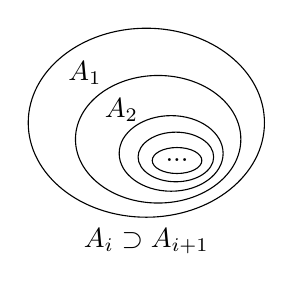
\begin{tikzpicture}[scale = 0.3]
		\draw (0,0) ellipse (5 and 4); 
		\draw (0.5,-0.7) ellipse (3.5 and 2.7);
		\draw (1.05,-1.3) ellipse (2.2 and 1.6);
		\draw (1.25,-1.45) ellipse (1.6 and 1.05);
		\draw (1.3,-1.6) ellipse (1.05 and 0.55);
		\node at (0,-5) {$A_i \supset A_{i+1}$};
		\node at (-2.6, 2.1) {$A_1$};
		\node at (-1.05,0.55) {$A_2$};
		\node at (1.3,-1.6) {$...$};
	\end{tikzpicture} 
}
\begin{defn}[Monotone sequence]
	A \textbf{monotone sequence} \marginleft{Monotone sequence: \\ $A_1 \subseteq A_2 \subseteq ...$\\ $A_1 \supseteq A_2 \supseteq ...$} is a sequence of sets $\{A_i\}_{i=0}^{\infty}$ where each set is a superset (or subset) of the preceding. More specifically, we distinguish four cases:
	\begin{description}
		\item[Increasing] when $A_i \subseteq A_{i+1}$ for all $i>0$
		\item[Decreasing] when $A_i \supseteq A_{i+1}$ for all $i>0$
		\item[Strictly increasing] when $A_i \subset A_{i+1}$ for all $i>0$
		\item[Strictly decreasing] when $A_i \supset A_{i+1}$ for all $i>0$
	\end{description}
\end{defn}

\begin{prop}[Monotone convergence]
	All monotone \marginleft{Monotone convergence} sequences converge. For increasing sequences the limit is given by $\lim\limits_{i \to \infty} A_i = \bigcup\limits_{i \geq 1} A_i$, while for decreasing sequences  the limit is given by $\lim\limits_{i \to \infty} A_i = \bigcap\limits_{i \geq 1} A_i$.
\end{prop}

\subsection{Homogeneous relations, equivalences and orders}

\begin{remark}
	We will cover the notions of orders that are necessary for the definition of ordinals and cardinal numbers. Orders will treated more in detail in a Bare Minimum dedicated to order theory.
\end{remark}

\begin{defn}[Homogeneous relation properties]
	Let $R \subseteq A \times A$ \marginleft{Reflexivity, symmetry, transitivity, ...} be a homogeneous binary relation between $A$ and itself. We define the following properties:
	\begin{description}
		\item[Reflexive.] Every element $a \in A$ is related to itself. That is, $aRa$ for all $a \in A$.
		\item[Irreflexive.] No element $a \in A$ is related to itself. That is, $aRa$ for no $a \in A$.
		\item[Symmetric.] If $a$ is related to $b$, then $b$ is related to $a$. That is, if $aRb$ then $bRa$.
		\item[Antisymmetric.] If $a$ is related to $b$ and $b$ is related to $a$, then $a$ and $b$ are the same element. That is, if $aRb$ and $aRb$ then $a=b$.
		\item[Transitive.] If $a$ is related to $b$ and $b$ is related to $c$, then $a$ is related to $c$. That is, if $aRb$ and $bRc$ then $aRc$.
		\item[Total.] Given two distinct elements, one is related to the other.That is, given $a \neq b$, either $aRb$ or $bRa$.
	\end{description}
	
\end{defn}

\begin{defn}[Orders and equivalence]
	A \textbf{partial order} (noted $\leq$, $\lesssim$, $\preceq$) \marginleft{Order, equivalence: $\leq$, $<$, $\equiv$} is a homogeneous binary relationship that is reflexive, antisymmetric and transitive. A \textbf{linear order} or \textbf{total order} is an order that is total. An order is \textbf{strict} (noted $<$, $\prec$) if it is irreflexive instead of reflexive.
	
	An \textbf{equivalence relation} (noted $\equiv$, $\sim$) is a homogeneous binary relationship that is reflexive, symmetric and transitive.
\end{defn}


\begin{defn}[Partitions]
	A \textbf{partition} \marginleft{Partitions} of a set $A$ is a collections $P \subset \mathcal{P}(A)$ of disjoint subsets that cover all of $A$. That is:
	\begin{enumerate}
		\item $\bigcup\limits_{B \in P} B = A$
		\item $B \cap C = \emptyset$ for all $B, C \in P$ where $B \neq C$
	\end{enumerate}
\end{defn}


\begin{defn}[Equivalence classes and quotient set]
	Let $A$ \marginleft{Eq. classes and quotient set: \\ $[a]_{\sim}, a_{/\sim}, A_{/\sim}$} be a set and $\sim$ an equivalence relation on $A$. Let $a \in A$. The \textbf{equivalence class of $a$ by $\sim$} is the set $[a]_{\sim} = a_{/\sim} = \{b \in A \, | \, b \sim a \}$ of all the elements of $A$ equivalent to $a$. The \textbf{quotient set of $A$ by $\sim$} $A_{/\sim} = \{ a_{/\sim} \, | \, a \in A \}$ all of the equivalences classes by $\sim$.
\end{defn}

\begin{prop}
	Every quotient set is a partition, and every partition is a quotient set. That is, let $A$ be a set and $\sim$ an equivalence class, then $A_{/\sim}$ is a partition. Conversely, let $P$ be a partition of $A$, then $\sim \; = \{ (a,b) \, | \, a, b \in X \text{ for some } X \in P \} $ is an equivalence relation and $A_{/\sim} = P$.
\end{prop}

\begin{defn}
	Given a function $f : A \to B$ the \textbf{equivalence relation determined by $f$} is the relation $R_f = \{ (a_1, a_2) \, | \, f(a_1) = f(a_2) \}$.
\end{defn}

\begin{prop}[Function canonical decomposition]
	Every function $f : A \to B$ can be written as the composition $f = t \circ s \circ r$ of the following three functions:
	\begin{description}
		\item[$r : A \to A_{/R_f}$] defined as $a \mapsto [a]_{R_f}$; this function is surjective
		\item[$s : A_{/R_f} \to f(A)$] defined as $[a]_{R_f} \mapsto f(a)$; this function is bijective
		\item[$t : f(A) \to B$] defined as $t(b) = b$; this function is injective.
	\end{description}
\end{prop}

%\begin{prop}[Set inclusion as ordering]
%	Set inclusion \marginleft{$\subseteq$ and $\supseteq$ are partial orders} (either $\subseteq$ or $\supseteq$) is a partial order. Strict set inclusion (either $\subset$ or $\supset$) is a strict partial order.
%\end{prop}

\subsection{Numeric constructions}
\begin{remark}
	The constructions that follow exemplifies the standard way numbers are defines in mathematics and it is useful to gain certain insights. In the Assumptions of Physics, however, we prefer to understand numbers as order-theoretic concept (i.e. the integer numbers can be thought as a linearly ordered set where each element have an immediate successor and an immediate predecessor).
\end{remark}
\begin{defn}\label{defn_successor_set}
	Let $A$ be a set. We define the \textbf{successor} $A^+ = A \cup \{A\}$. A set $S$ is called a \textbf{successor set} if it contains the empty set (i.e. $\emptyset \in S$ and if contains the successor of every element (i.e. if $X \in S$ then $X^+ \in S$). The set of \textbf{natural numbers} $\mathbb{N}$ is the intersection of all successor sets.
\end{defn}
\begin{remark}
	The natural numbers so constructed are known as von Neumann ordinals. They are as follows:
	\begin{itemize}
		\item $0 = \{ \} = \emptyset$
		\item $1 = \{ 0 \} = \{ \emptyset \}$
		\item $2 = \{0, 1\} = \{ \emptyset, \{ \emptyset\} \}$
		\item $3 = \{0, 1, 2\} = \{ \emptyset, \{ \emptyset\}, \{ \emptyset, \{ \emptyset\} \} \}$
		\item $4 = \{0, 1, 2, 3\} = \{ \emptyset, \{ \emptyset\}, \{ \emptyset, \{ \emptyset\} \}, \{ \emptyset, \{ \emptyset\}, \{ \emptyset, \{ \emptyset\} \} \} \}$
		\item ...
	\end{itemize}
	It can be shown that they obey Peano's axioms, another common way to axiomatize the natural numbers and their arithmetic.
\end{remark}

\subsection{Ordinal numbers}

For infinite sets, cardinals and ordinals are different since sets of the same infinite size can be given different orderings. 

\begin{remark}
	Cardinal numbers (i.e. one, two, three, ...) identify the number of elements in a set. Ordinal numbers (i.e. first, second, third) identify a position within a sequence. Well-ordered sets extend the notion of sequence to arbitrary levels of infinity.
\end{remark}

\begin{defn}[POS]
	A \textbf{partially ordered set}, \marginleft{POS: $(A, \leq_A)$} or \textbf{POS}, is a tuple $(A, \leq_A)$ where $A$ is a set and $\leq_A$ is a partial order over $A$. A \textbf{linearly ordered set} is a POS whose order is linear.
\end{defn}

\begin{defn}[Initial segment]
	The \textbf{initial segment} \marginleft{Initial segment} of a POS $(A, \leq_A)$ determined by $a \in A$ is the set of all elements less than $a$. That is, $S_a=\{ x \in A \, | \, x < a \}$.
\end{defn}

\begin{defn}[Order morphisms]
	Let $(A, \leq_A)$ \marginleft{Order homo/ \\ isomorphism} and $(B, \leq_B)$ be two POSs. An \textbf{order homomorphism} is a function $f : A \to B$ that preserves the ordering. That is, $a_1 \leq_A a_2$ implies $f(a_1) \leq_B f(a_2)$. An \textbf{order isomorphism} is a bijective order homomorphism whose inverse is also an order homomorphism. That is, $b_1 \leq_B b_2$ implies $f^{-1}(b_1) \leq_A f^{-1}(b_2)$.
\end{defn}

\begin{defn}[Well-order]
	A \textbf{well-ordered} \marginleft{Well-order} set is a linearly ordered set $(A, \leq_A)$ where each subset has a least element. That is, for every $B \subseteq A$, there exists an $a \in B$ such that $a \leq_A b$ for all $b \in B$. Let $A$ and $B$ be two well ordered set, we say $A$ \textbf{has lower ordinality than} $B$, noted $A \ordleq B$, if $A$ is order isomorphic to an initial segment of $B$. They have \textbf{the same ordinality}, noted $A \ordeq B$, if they are order isomorphic.
\end{defn}

\begin{prop}[Ordinality]
	If $A$ and $B$ are two well ordered sets, then either $A \ordleq B$ or $B \ordleq A$. If $\mathcal{A}$ is a collection of well-ordered sets, then one element has least ordinality.
\end{prop}

\begin{remark}
	Examples of well-ordered sets:
	\begin{itemize}
		\item a finite sequence: $(a_1, a_2, ..., a_n)$
		\item an infinite sequence: $(a_1, a_2, ..., a_n, ...)$
		\item an infinite sequence with elements afterwards: $(a_1, a_2, ..., a_n, ..., b_1, b_2, ... , b_6)$
	\end{itemize}
	In a well-ordered set, every element always has an immediate successor, but not necessarily an infinite predecessor (e.g. $b_1$ in the third example). 
\end{remark}

\begin{remark}
	Ordinal numbers generalize the construction of von Neumann ordinals and cover all possible positions in well-ordered sets.
\end{remark}

\begin{defn}[Ordinals]
	An \textbf{ordinal} \marginleft{Ordinals: \ordinals} is a set $A$ with the following properties for all $a, b, c \in A$:
	\begin{enumerate}
		\item $a \notin a$
		\item $a \in b$ implies $b \notin a$
		\item $a \in b$ and $b \in c$ implies $a \in c$
		\item $x \in a$ implies $x \in A$
	\end{enumerate}
	We note $\ordinals$ as the class of all ordinals.
\end{defn}

\begin{prop}[Ordinals are well-ordered]
	Let $a \in \ordinals$ be an ordinal. Then $(a, \in)$ is a well-ordered set.
\end{prop}

\begin{prop}[Ordinality of a well-ordered set]
	For every \marginleft{$\langle A \rangle$} well-ordered set $A$ there is a unique $\langle A \rangle \in \cardinals$ such that $a \ordeq A$. We say $\langle A \rangle$ is the \textbf{ordinality of $A$}. The natural numbers are the initial segment of the ordinals. $\omega$ is the ordinal associated with the natural numbers.
\end{prop}

\begin{remark}
	As an example, consider the von Neumann ordinal $3 = (0, 1, 2)$ as a well-ordered set. We can see it as a sequence of three element, which means the last is the third. Similarly, the ordinality of the set $(a_1, a_2, a_3)$ is $3 = (0, 1, 2)$ as they define well-ordered set with the same ordering. The definitions are such that these ideas extend to infinite sets.
\end{remark}

\begin{defn}[Ordinal addition]
	Let $(A, \leq_A)$ \marginleft{Ordinal addition: $\langle A \rangle + \langle B \rangle$} and $(B, \leq_B)$ be two well ordered sets. Let $(A \sqcup B, \leq)$ be the POS where:
	\begin{itemize}
		\item $(A, a_1) \leq (A, a_2)$ if $a_1 \leq_A a_2$
		\item $(B, b_2) \leq (B, b_2)$ if $b_1 \leq_B b_2$
		\item $(A, a) \leq (B, b)$ for all $a \in A$ and $b \in B$.  	
	\end{itemize}
	Then $(A \sqcup B, \leq)$ is well-ordered and the ordinal $\langle A \sqcup B \rangle$ is fully determined by $\langle A \rangle$ and $\langle B \rangle$. Therefore we can define the \textbf{ordinal addition} $\langle A \rangle + \langle B \rangle =  \langle A \sqcup B \rangle$.
\end{defn}

%\begin{prop}[Ordinal multiplication]The addition has the following properties:
%	\begin{enumerate}
%		\item associative: $\langle A \rangle + ( \langle B \rangle + \langle C \rangle) = (\langle A \rangle + \langle B \rangle) + \langle C \rangle$
%		\item $\langle 0 \rangle = \langle \emptyset \rangle$ is the identity: $\langle A \rangle + \langle 0 \rangle = \langle 0 \rangle + \langle A \rangle = \langle A \rangle$
%		\item not commutative in general: $\langle A \rangle + \langle B \rangle$ not necessarily the same as $\langle B \rangle + \langle A \rangle$
%		\item reduces to arithmetic addition on the natural numbers
%	\end{enumerate}
%\end{prop}

\begin{remark}
	Addition in non-commutative (i.e. $\langle A \rangle + \langle B \rangle \neq \langle B \rangle + \langle A \rangle$) for infinite ordinals. For example $(a_1, a_2, ..., a_n, ...) \sqcup (b_1, b_2, b_3) = (a_1, a_2, ..., a_n, ..., b_1, b_2, b_3)$ is not the same as $(b_1, b_2, b_3) \sqcup (a_1, a_2, ..., a_n, ...) = (b_1, b_2, b_3, a_1, a_2, ..., a_n, ...) \simeq (c_1, c_2, ..., c_n, ...)$. Therefore $\omega + 3 \neq 3 + \omega = \omega$.
\end{remark}

\begin{defn}[Ordinal multiplication]
	Let $(A, \leq_A)$ \marginleft{Ordinal multiplication: $\langle A \rangle \langle B \rangle$} and $(B, \leq_B)$ be two well ordered sets. Let $(A \times B, \leq)$ be the POS where:
	\begin{itemize}
		\item $(a_1, b_1) \leq (a_2, b_2)$ if $b_1 \leq_B b_2$
		\item $(a_1, b) \leq (a_2, b)$ if $a_1 \leq_A a_2$
	\end{itemize}
	Then $(A \times B, \leq)$ is well-ordered and the ordinal $\langle A \times B \rangle$ is fully determined by $\langle A \rangle$ and $\langle B \rangle$. Therefore we can define the \textbf{ordinal multiplication} $\langle A \rangle \langle B \rangle =  \langle A \times B \rangle$.
\end{defn}

%\begin{prop}[Ordinal multiplication]
%	The multiplication has the following properties:
%	\begin{enumerate}
%		\item associative: $\langle A \rangle ( \langle B \rangle \langle C \rangle) = (\langle A \rangle \langle B \rangle) \langle C \rangle$
%		\item $\langle 1 \rangle = \langle \{ \emptyset \} \rangle$ is the identity: $\langle A \rangle \langle 1 \rangle  = \langle 1 \rangle \langle A \rangle = \langle A \rangle$
%		\item right distributive over addition: $\langle A \rangle ( \langle B \rangle + \langle C \rangle) = \langle A \rangle \langle B \rangle + \langle A \rangle \langle C \rangle$
%		\item $\langle A \rangle \langle 0 \rangle  = \langle 0 \rangle \langle A \rangle = \langle 0 \rangle$
%		\item not commutative in general: $\langle A \rangle + \langle B \rangle$ not necessarily the same as $\langle B \rangle + \langle A \rangle$
%		\item reduces to arithmetic multiplication on the natural numbers
%	\end{enumerate}
% The multiplication is associative and $\langle \emptyset \rangle$ is the identity (i.e. $\langle A \rangle + \langle \emptyset \rangle = \langle \emptyset \rangle + \langle A \rangle = \langle A \rangle$). The additions is not, in general, commutative.
%\end{prop}

\begin{remark}
	Muliplication is non-commutative (i.e. $\langle A \rangle \langle B \rangle \neq \langle B \rangle \langle A \rangle$) for infinite ordinals. For example $(a_1, a_2, ..., a_n, ...) \times (b_1, b_2) = ((a_1, b_1), (a_2, b_1), ..., (a_n, b_1), ..., \\ (a_1, b_2), (a_2, b_2), ..., (a_n, b_2), ...)$ is not the same as $(b_1, b_2) \times (a_1, a_2, ..., a_n, ...) = ((b_1, a_1), (b_2, a_1), (b_1, a_2), (b_2, a_2), ..., (b_1, a_n), (b_2, a_n), ...) \simeq (c_1, c_2, ..., c_n, ...)$. \\ Therefore $\omega 2 \neq 2 \omega = \omega$.
	
	With addition and multiplication, we can get a sense of how the ordinals work. $\omega$ represents a countable sequence. $\omega +3$ is a countable sequence followed by three elements. $\omega + \omega  = \omega2$ represents a countable sequence followed by a countable sequence. $\omega6$ represents a sequence of 6 countable sequences. $\omega\omega = \omega^2$ represents a countable sequence of countable sequences. $\omega^3$ represents a countable sequence of countable sequences of countable sequences. $\omega^\omega$ extends the recursion infinitely many times and so on. There is no upper limit to the ordinals.
\end{remark}

\begin{remark}
	The cardinality of a set (i.e. how many elements it contains) is defined in terms of injection/bijection: a set is smaller than another if it can be injected into it, and it is as big as another if it can be put into a one-to-one correspondence.
\end{remark}

\begin{defn}[Cardinal comparison]
	Let $A$ \marginleft{Cardinality} and $B$ be two sets. If there exists a injective function $f : A \to B$ then we say $A$ \textbf{has lower cardinality than} $B$, noted $A \crdleq B$. If there exists a bijective function we say they have \textbf{the same cardinality}, noted $A \crdeq B$.
\end{defn}

\begin{prop}[Cardinal comparability of sets]
	Given two sets $A$ and $B$, either $A \crdleq B$ or $B \crdleq A$ one must have lower cardinality than the other (i.e. there exists an injective function from one two the other). Additionally, $A \crdeq B$ if and only if $A \crdleq B$ and $B \crdleq A$ (i.e. there exists a bijective function between $A$ and $B$ only if there exists an injective function in both direction).
\end{prop}

\begin{prop}[Well-ordering theorem]
	Every set can be well-ordered.
\end{prop}

\begin{remark}
	The well-ordering theorem allows us to reuse ordinal numbers to quantify cardinality. As two different well-ordered sets may have the same cardinality, we'll take the lowest ordinal between them.
\end{remark}

\begin{defn}[Cardinal number]
	A \textbf{cardinal}  \marginleft{Cardinals: $\cardinals$} is an ordinal $a \in \ordinals$ that has lower ordinality of any ordinal that has the same cardinality. That is, $a \ordleq b$ for all $b \in \ordinals$ such that $a \crdeq b$. The set of all cardinals is noted $\cardinals \subset \ordinals$.
\end{defn}

\begin{prop}[Cardinality of a set]
	For every \marginleft{$|A|$} set $A$ there is a unique $|A| \in \cardinals$ such that $a \crdeq A$. We say $|A|$ is the \textbf{cardinality of $A$}.
\end{prop}

\begin{remark}
\end{remark}

\section{Axiomatic set theory}

Introduce paradoxes. Axiomatic set theory is a family of attempt to solve those paradoxes. There are different variations.

Formalization to remove semantic paradoxes. All approaches of axiomatic set theory do that.

%https://en.wikipedia.org/wiki/Zermelo%E2%80%93Fraenkel_set_theory

%https://en.wikipedia.org/wiki/Von_Neumann–Bernays–Gödel_set_theory

\subsection{Classes, sets and elements}

As some collections cannot \marginright{TODO: diagram with Classes, proper classes and sets.} be put into other collections without creating paradoxes, the resolution of syntactic paradoxes is through the distinction between classes and sets. Classes are all those objects that can contain elements. Sets are particular classes that can also be elements of other classes. Therefore we can have the class of all sets, but we cannot have the set of all sets or the class of all classes.

\subsection{Axiomatization}

There are different approaches to the axiomatization of set theory with different degree of variation. One strategy, refered to as Zermelo–Fraenkel (ZFC), only defines sets. It avoids paradoxes by restricting set construction to subsets only.

Another strategy, refered to as von Neumann–Bernays–Gödel (NBG), starts by defining classes and then defines sets as those classes that can be elements of classes. It avoids paradoxes by restricting set construction on predicates over elements. Since a proper class is not an element, if the definition creates a contradiction for an item $x$ (i.e. we have both $x \in S$ and $x \notin S$) than it must be that the element $x$ is a proper class.

\textbf{Axioms}. Here are the axioms of a particular formulation of axiomatic set theory taken from CITE:
\begin{enumerate}
	\item Axiom of extent. If two classes have the same elements, then they are identical.
	\item Axiom of class construction. Let $P(x)$ be a predicate expressed in terms of the symbols $\in, \OR, \AND, \NOT, \Rightarrow, \exists, \forall$, brackets, variables $x, y, z, A, B, ...$ Then there exists a class $C$ that consists of all the elements x which satisfy $P(x)$.
	\item Every subclass of a set is a set.
	\item $\emptyset$ is a set.
	\item If $a$ and $b$ are sets, then $\{a, b\}$ is a set.
	\item If $\mathcal{A}$ is a set of sets, then, $\bigcup\limits_{A \in \mathcal{A}} A$ is a set.
	\item If $A$ is a set, the power set $\mathcal{P}(A)$ is a set.
	\item Axiom of foundation. If $A \neq \emptyset$ is a set, there exists an element $a \in A$ such that $a \cap A = \emptyset$.
	\item Axiom of replacement. If $A$ is a set and $f : A \to B$ is a surjective function, then $B$ is a set.
	\item Axiom of choice. Every set has a choice function. That is, given a set $A$, there exists a function $f : \mathcal{P}(A) \setminus \{ \emptyset \} \to A$ such that $f(B) \in B$.
	\item Axiom of infinity. There exists a successor set (as defined in \ref{defn_successor_set}).
\end{enumerate}

Cardinal numbers

\begin{prop}[Well-ordering theorem]
	Every set can be well-ordered.
\end{prop}

Define ordering by existence of injection.

def equipotent set (bijective)

prop no surjective funtion from a to P(A)

talk about contiunuum hypo as example of work in set theory


\begin{remark}
	Axiom 1 serves to define class equality. Axiom 2 defines how to define classes based on predicates. Axioms 3-7 tells us that some classes, constructable by axiom 2, are sets. Axiom 8 guarantees that we cannot have an infinite sequences $\{ A_i \}_{i=1}^\infty$ such that $A_{i+1} \in A_i$. In particular, a set cannot be an element of itself. Axiom 9 tells us that any set that is ``smaller'' than a set (i.e. we can map another set onto it) is a set. Axiom 10 guarantees that we can always pick an element from a set, though it does not tell us how. Axiom 11 tells us that there are sets with infinite elements.
\end{remark}

Ugly elements of set theory: all mathematical objects are sets. Numbers are set.


%\bibliographystyle{plain}
%\bibliography{bibliography}

\end{document}